In the following section, visualizing is meant to be about visualizing the structure, and not about visualizing what neural networks see.\cite{deepnetworkvisualizing2015}

Traditional neural networks are relatively easy to visualize.

An example of this is such a network with two inputs, three hidden neurons and one output neuron.

{\centering
	\begin{neuralnetwork}[height=3, nodespacing=1.5cm]
		\newcommand{\nodelabel}[2]{
			\ifnum#1=0 $x_#2$ \fi
			\ifnum#1=1 $y_#2$ \fi
			\ifnum#1=2 $z_#2$ \fi
		}
		\setdefaultnodetext{\nodelabel}
		\inputlayer[count=2, bias=false, title=]
		\hiddenlayer[count=3, bias=false, title=] \linklayers
		\outputlayer[count=1, title=] \linklayers
	\end{neuralnetwork}
	\par}

For us, the minimum of visible structure for a neural network to be readable is knowledge of the input layer location, the neurons (displayed as circles) and the connections, displayed as lines.

Additional information that we found useful in understanding the network would be showing the exact weight of the connections.

We created a algorithm to calculate the scaling of the differently sized networks automatically for a fixed space:

For this algorithm, we need information about the amount of layers, the max amount of neurons in any layer.

For the definition of the algorithm, we simply assume the the network will be shown from left to right, with all input-neurons to the left.

The x-axis below is defined horizontal, the y axis vertical.

$ width $ is the available width (also $ xSize $), $ height $ is the available height (also $ ySize $).

$ layerCount $ is defined as the amount of layers, $ maxNeuronCount $ as the max amount of neurons in any layer.

A $ Step $ (x or y) defines the distance between the centers of neurons, in x or in y direction, respectively.

$$ xStep = (xSize - ((layerCount + 2) * (minMargin + neuronRadius * 2))) $$

$$ yStep = (ySize - ((maxNeuronCount + 2) * (minMargin + neuronRadius * 2))) $$

 whereat $ minMargin $ is the margin that should be kept between neurons to make sure they aren't overlapping, and $ neuronRadius $ is the radius of the neurons to be drawn.
 
 $ layerCount + 2 $ is there, because there are also borders to be kept at the corner of the drawing area to be drawn on - exactly 2 per dimension.
 
 Of course, this means that if $ (minMargin + neuronRadius) * (layerCount + 2) > width $ the neurons will overlap anyways and the structure will be hard to read.
 
 This will result in such a structure (taken straight from our software NEAT\_Visualizer):
 
 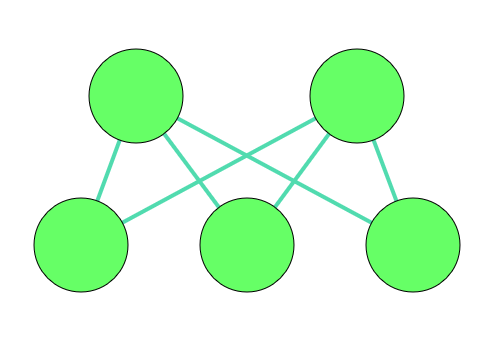
\includegraphics[scale=0.5, angle=90]{visualizer.png}